\documentclass{article}
\usepackage{amsmath}
\usepackage{graphicx} % gráficos
\usepackage[noblocks]{authblk}
%\usepackage{float}
%\usepackage{cite}% para contraer referencias
%\usepackage[usenames]{color}
\usepackage{bm}
\usepackage{ulem} %opcional para la correcciones
\newcommand{\abs}[1]{\lvert#1\rvert}
\usepackage{xcolor}
\newcommand{\notaL}[1]{{\color{blue}+L:#1+}}
\newcommand{\notaC}[1]{{\color{green}+C:#1+}}
\newcommand{\notaV}[1]{{\color{red}+V:#1+}}
\title{\textbf{Optimization of Porous Silicon Gradient Refractive
    Index Structures.} }
% A comparison with computational schemes with experimental results
\author[1]{C. A. Ospina de la Cruz}
\author[2]{W. L. Mochán }
\author[3]{V. Agarwal }

\affil[1]{Posgrado en Ingenier\'ia y Ciencias Aplicadas del Centro de
  Investigación en Ingenier\'ia y Ciencias Aplicadas (CIICAp-IICBA),
  Universidad Autónoma del Estado de Morelos (UAEM), Cuernavaca CP
  62209, México}
\affil[2]{Instituto de Ciencias F\'isica ,Universidad Nacional
  Autonoma de Mexico, Av. Universidad S/N, Col. Chamilpa, 62210
  Cuernavaca, Morelos, Mexico}
\affil[3]{Centro de Investigaci\'on en Ingenier\'ia y Ciencias
  Aplicadas,Universidad del Estado de Morelos, Av. Universidad 1001
  Col. Chamilpa, Cuernavaca, Morelos 62209, Mexico  }
\begin{document}

\maketitle

\begin{abstract}
We propose a simple setup which that the calculation of the current
density as a function of position within an electrochemical cell used
to produce porous Silicon structures with a controlled gradient in their
index of refraction. We produced samples under several conditions and
characterized them with scanning electron microscopy, and
ultraviolet-visible-near infrared reflectance spectroscopy. Our
results allow us to obtain from experiments on a single or just a few
samples a full characterization of the dependence of porosity,
dielectric function and speed of attack on the current density and on
position, so that novel nonhomogeneous devices may be designed and
built.

Keywords: Porous Silicon; GRIN; Reflectance Spectra.
\end{abstract}
\notaL{Cambié el abstract, pero habrá que revisarlo después.}
\notaL{Si quieres ponerme algún comentario en el manuscrito usa el
  comando notaC, similar al comando notaL que uso yo}
\section{Introduction}
\label{sec:introduction}
\notaL{Debiste poner etiquetas en todas las subsecciones y secciones, y
  ecuaciones y figuras.}
\notaL{No entiendo nada de la introducción}
The structural properties of nanostructured materials  has  received a
considerable attention,  and a large research effort has been devoted
to them \cite{I1}. We found a great way to go for future
technological  explorations,  countless  challenges and  that  open a
range of possibilities to develop further  study  on these
issues\cite{I2}. Porous silicon (PS) is a versatile nanostructured
material and an excellent candidate as a technological platform for
different sensing applications \cite{I3, I4}, due to its easy
manufacturing,  large surface area, high surface reactivity,  and
moreover, its optical transduction capacity.  Photonic crystals are
multilayer dielectric structures that have periodicity in the
dielectric function along one direction \cite{I5}. It has numerous
studies for high reflectivity and the ability to adjust  the photonic
prohibited  band (PBG)\cite{I6} , which leads to possible applications
such as filters\cite{I7}, optical switches\cite{I8}, omnidirectional
mirrors\cite{I9}, waveguides for PC \cite{I10} etc. In the
conventional manufacturing of PS the desired result  is to obtain
homogeneous samples (same structural characteristics) from the
periphery  to the center  of the electrochemically  attacked area.
However, with an asymmetric anodizing configuration,  samples with a
lateral gradient in terms of pore size and thickness of the porous
layer are obtained \cite{I101}. In this configuration,  the face of
the platinum  electrode (cathode)  is relatively maintained
perpendicular  to the surface of the Si substrate (anode) at one end
of the cell, so that the distribution of the current within the
electrolyte  solution varies depending on the distance  of the
electrode due to the resistance of the electrolyte,  resulting  in a
decrease in current density as the distance from the electrode
increases \cite{I102, I103}. The result is a porous surface with
different pore sizes ranging from a few nanometers  to pores on the
order of a few micrometers  \cite{I104}. The dimensions of the pores
obtained on the same chip can be controlled by adjusting the anodizing
current and electrolyte concentration \cite{I11}. Currently, these
types of samples have found their application relevant as optical band
filters \cite{I12}, devices with a multidirectional photonic band
(photonic bar codes) \cite{I13} and mainly as biosensors. In this way,
the effect of different topographies (porosities in the same sample)
on the culture / adhesion of certain cells \cite{I14} is studied,
considerably reducing the number of samples and cost of the study. In
addition, they are also very useful when a biomolecule size-exclusion
technique is required allowing the identification and separation of
these biological compounds \cite{I15}. Recent studies  have shown that
the  combination  of thermal  oxidation  and infiltration of TiO2   by
ALD offers the  opportunity to manufacture  a high index of refraction
of contrast, visibly transparent GRIN optical elements from PS
absorbent structures \cite{I16}. A Despite previous research on the
formation of porous silicon with GRIN, type p in manufacturing and
characterization, there was no control of current densities, much less
a model that  explained said lateral  gradient. In this work, we
reported a gradient refractive index (GRIN) structure by varying the
current density on the fabrication of porous silicon photonic
structure. This current density values, depth, and porosity of the
photonic structure were calculated from an electrostatic model for
photonic crystals with a gradient refractive index
(EMPCGRIN). Moreover, the theoretical and experimental studies were
exhibited similar results.

The paper is organized as follows. In Section 2  we report the effect
of how the current density can be calculated from an electrostatic
model for photonic crystals with gradient refractive index (EMPCGRIN),
demonstrating that there is a direct relation of the gradient
generated by the electrode when it attacks the Silicon sample, we can
see the depth of the structure and its porosity, in each of the
measuring points. In Subsection 2.2 we present a formalism based on
the methods used for the analysis of photonic crystal structures is
the transfer matrix method. We use it to investigate the reflectance
of light in a one-dimensional photonic crystal. In Section 3 we
provide experimental  details about the manufacture of PS dielectric
multilayers and Section 4 we shows the comparison of numerical and
experimental results followed. Finally,  the conclusions given in
Section. 5

\section{Theory} \label{sec:theory}
\subsection{Calculation of the current density}
\label{sec:calc-curr-dens}
\notaL{check where acronyms are first defined}
A gradient in the optical properties of porous Silicon (PS) systems may be
obtained by electrochemically attacking a Si surface with a position dependent current
density ${\bm j(\bm r)}$, as the porosity and refractive index depend on
the current density, as well as the speed of attack and the thickness of the
porous layer. Nevertheless, it is not a simple task to measure the
{\em local} value of $\bm j(\bm r)$ along the surface. This hampers the
design and optimization of well characterized reproducible GRIN PS
structures.\notaL{Tenemos referencias para afirmar esto?} Thus, we
believe a
system for which the current density field may be
easily computed would be useful.
Though $\bm j(\bm r)$ may be in principle be numerically calculated for a
given arbitrary experimental setup,  here we propose a particularly
simple setup that allows an expression for the current in terms
of a series that is rapidly convergent and each of whose terms is a
simple analytic function. With this setup it is easy to characterize
the dependence of different properties of interest on the current, and
this allows the design and optimization of diverse GRIN PS devices.

We assume that our electrolytic cell has the shape of a
prism (see Fig. \ref{f:celda}) with a horizontal rectangular base of sides $a$ and $b$, and
filled with the electrolyte up to a height $c$. We assume that the
walls of the cell are insulating while the bottom is completely
covered with the sample, which is a which is an
electrically grounded good conductor. Within the electrolyte we position an electrode
which we assume is a thin conductor, insulated from the electrolyte
but for a small area near its tip, which we thus approximate as a
point current source.
\begin{figure}
  \centering
  \includegraphics[width=\textwidth]{Images/celdan1}
  \caption{Prism shaped electrolytic cell with a rectangular base of
    sides $a$, $b$ filled with electrolyte up to a height $c$. The
    walls of the cell are insulating and the bottom is completely
    covered by the sample, which is assumed to be a good
    conductor. The tip of the electrode is a thin insulated wire
    \notaL{El punto del electrodo hazlo más chico que el ancho
      del cable.} with just the tip uncovered and located at $\bm r_0=(x_0,y_0,z_0)$ within the
    liquid.}
  \label{f:celda}
\end{figure}
Within the electrolyte the current density is
\begin{equation}
  \label{eq:j}
  \bm j=\sigma\bm E,
\end{equation}
with
$\sigma$ the conductivity, $\bm E=-\nabla\phi$ the electric field,
and $\phi$ the electric potential. For a
stationary situation\notaL{Latex usa nabla como el nombre de
  $\nabla$}
$\nabla\cdot \bm j = \sigma\nabla\cdot\bm E=0$. Thus, within the electrolyte,
\begin{equation}
  \label{eq:laplace}
\nabla^{2} \phi=0.
\end{equation}
Consider now an arbitrary closed surface
$\mathcal S$
within the electrolyte that surrounds completely the tip of the
electrode. Integrating $ \bm j$ over this surface we obtain
\begin{equation}
  \label{eq:I}
\int_{\mathcal S'} d\bm a \cdot \bm j = -I,
\end{equation}
where the prime on $\mathcal S'$ means we remove from the surface a
very small hole through which the wire that feeds the current to the
electrode gets
through. Assuming the wire is narrower than any other relevant
distance in the system, we may interpret Eq. \eqref{eq:I} as an
integral over a closed surface of the current \eqref{eq:j} within the
electrolyte, ignoring the actual current within the wire. Thus
\begin{equation}
  \label{eq:gauss}
  \int_{\mathcal S} d\bm a \cdot \bm E = -\frac{I}{\sigma}
\end{equation}
Using Gauss's law, we interpret this equation as a source for the
potential in the form of a point charge
\begin{equation}
  q_0 = -\frac{I}{4 \pi \sigma}
\end{equation}
at the position $\bm r_0=(x_0, y_0, z_0)$ of the
tip of the electrode. Note that $q_0$ would be the total charge,
and it shouldn't be further screened through the permittivity of the
electrolyte.

The effective conductivity of the relatively thin sample in contact
with the grounded counterelectrode is large enough that we may assume its
surface $z=0$ is an equipotential.
On the other hand, no current can go across the insulating walls of
the cell, situated at $x=0$, $x=a$,, $y=0$ and $y=b$, nor through the
free surface of the liquid at $z=c$. Thus, the problem to solve is Poisson's
equation with a point charge source
\begin{equation}
  \label{eq:poisson}
  \nabla^2\phi=-4\pi q_0\delta(\bm r-\bm r_0),
\end{equation}
with mixed boundary conditions
\begin{equation}
  \label{eq:ground}
  \phi(x,y,0)=0,
\end{equation}
and
\begin{equation}
E_x(0, y ,z)= E_x(a, y ,z)=E_{{_y}}(x, 0 ,z)=E_{{_y}}(x, b
,z)=E_{{_z}}(x, y ,c)=0.
\end{equation}
This problem may be solved readily using image charge theory \cite{T1,T2}.
The potential within the electrolytic cell coincides
within the region $0\le x\le a$, $0\le y \le b$, $0\le z\le c$
with that an infinite fictitious empty space but for the point charge
$q_0$ at the tip of the electrode at $\bm r_0$, and an array of its fictitious image
charges. The images include a reflection on the conducting bottom of the
cell, of the opposite charge $-q_0$ and situated at $(x_0, y_0,-z_0)$,
to guarantee that the bottom stays at potential zero.
There are further images on the four walls of the cell, of the same charge $q_0$
and situated at $(-x_0,Y_0,z_0)$, $(x_0,-y_0, z_0)$, $(2a-x_0, y_0,
z_0)$ and $(x_0, 2b-y_0,z_0)$ to guarantee that no current goes across
them. Similarly, there is an image of the same charge $q_0$ at
$(x_0,y_0,2c-z_0)$ to guarantee that no current goes across the
surface of the electrolyte. Furthermore, each image charge has to be
further reflected by each of the aforementioned surfaces, yielding new
images.
\begin{figure}
  \centering
  \includegraphics[width=\textwidth]{paper-1}
  \caption{Top view of the fictitious system formed by reflections of
    the electrolytic cell (light blue) showing the charge at the
    tip of the electrode (red dot) and its images on the walls of the
    rectangular cell, the images of its images and so on (blue
    dots). The walls are at $x=0,a$,
    $y=0,b$ (blue lines). The relation of some charges and their images is
    indicated by dashed arrows, with a bar to indicate the
    corresponding reflecting wall. The system may be interpreted as a
    periodic lattice with a rectangular unit cell of size $2a\times 2b$,
    one of which is indicated  by wide dashed lines, and with a basis of four equal
    charges $q_0$ at $(\pm x_0, \pm y_0, z_0)$.}
  \label{fig:topview}
\end{figure}
In Fig. \ref{fig:topview} we illustrate the real charge and all of
its images within the plane $z=z_0$. They form a periodic rectangular
lattice with a unit cell of size $2a\times 2b$ and with a basis of
four equal charges $q_0$ situated at the positions $\bm r_0$, $\bm
r_1=(-x_0, y_0, z_0)$, $\bm r_2=(x_0, -y_0, z_0)$ and $\bm r_3=(-x_0,
-y_0, z_0)$. In Fig. \ref{fig:sideview} we show a lateral view of the
image charges.
\begin{figure}
  \centering
  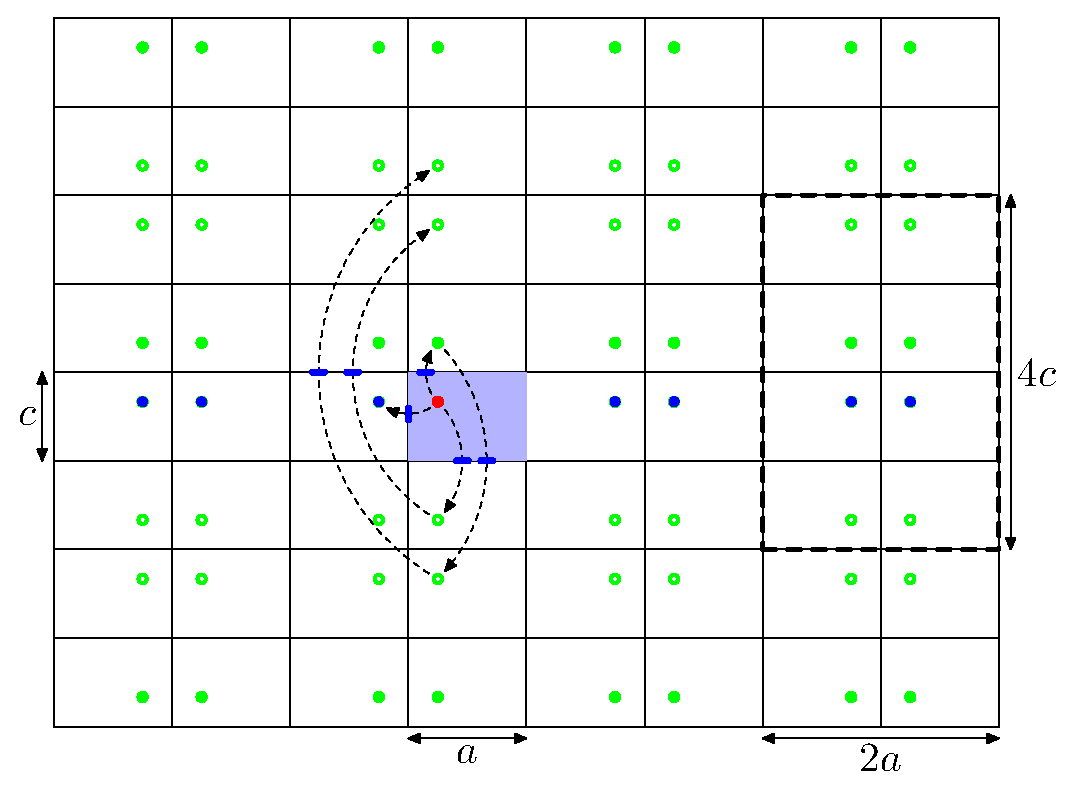
\includegraphics[width=\textwidth]{paper-2}
  \caption{Side view of the fictitious system formed by reflections of
    the electrolytic cell (light blue)
    showing the charge at the tip of the electrode (red dot), its
    images within the plane $z=z_0$ (blue dots), and its images at the
    surface of the sample and the top of the electrolyte (green
    dots). We use solid dots to denote images with the same charge $q_0$
    as that corresponding to the tip of the electrode, and open dots for those of
    opposite charge $-q_0$. The mirror planes that don't invert the charge
    are indicated by blue lines and the mirror plane that inverts the
    charge is indicated by a red line. The relation of some charges and their images is
    indicated by dashed arrows, with a bar to indicate the
    corresponding reflecting wall. The system may be interpreted as a periodic
    lattice with a rectangular unit cell of size $2a\times 4c$, one of
    which is indicated by wide dashed lines, and with a basis of four
    charges $q_0$ and another four charges $-q_0$. Within this cell,
    we indicate its $G=0$ contribution to the electric field (solid
    arrows, see text).}
  \label{fig:sideview}
\end{figure}
Each plane of charges upon reflection on the surface of the sample at
the bottom of the cell yields an
plane of image charges of the opposite sign, while reflections
on the surface of the liquid yields a plane of charges of the same
sign. The side view may be interpreted as a periodic rectangular
lattice with a unit cell of size $2a\times 4c$ containing a basis of eight point
charges, four positive and four negative. A projection onto the $yz$
plane would similarly yield a rectangular lattice with a  $2b\times4c$
unit cell. Putting everything together, the problem is that of solving
Poisson's equation within an orthothombic lattice of size
$2a\times2b\times4c$ with a basis of 16 point charges of charge $\pm
q_0$ arranged in positive and negative planes.

The electrostatic potential produced by an infinite array of
charges expressed as a sum in real space of Coulomb terms has ill
convergence properties. The potential can be obtained
using the Ewald summation technique \cite{T3,T4,T5}, which yields
two rapidly converging series, one in real space and another one in reciprocal space.
Nevertheless, as we need the potential and the field to obtain the
current density on the surface of the sample on which there are no
real nor image charges, we may perform a somewhat simpler planewise
summation, where we first obtain the potential and field produced by a
simple periodic lattice of charges using a fast convergent sum over the 2D
reciprocal vectors, then sum over the charges that form the basis
of the 2D {\em crystal} plane, and finally sum over all the
 planes \cite{T6,T7}.

We consider first a system made of identical unit charges
ocuppying the positions $\bm R$ of a 2D Bravais lattice $\{\bm R\}$,
which we will take as a rectangular lattice with lattice parameters
$2a$ and $2b$, and lying, for the time being, at the $z=0$ plane.
The potential it produces obeys
\begin{equation}
  \label{eq:poissonRed}
  \nabla^2\phi(\bm r)=-4\pi\sum_{\bm R}\delta(\bm r_\|-\bm
  R)\delta(z)=-\frac{4\pi}{A}\sum_{\bm G}e^{i\bm G\cdot\bm r_\|}\delta(z),
\end{equation}
where $\bm r_\|$ is the projection of the observation position $\bm
r=(x,y,z)$ onto the $xy$ plane,
$\delta(\ldots)$ is Dirac's delta function, $\{\bm G\}$ is the
reciprocal lattice defined through $e^{i\bm G\cdot\bm R}=1$ for all
$\bm R$ and $\bm G$, $A=4ab$ is the area of the unit cell
and we used the Fourier representation of the 2D
periodically repeated delta function. We introduce a 2D Fourier representation for
the potential \notaL{\sout{Checar consistencia entre phi y varphi en todos lados}}
\begin{equation}
  \label{eq:phifourier}
  \phi(\bm r)=\sum_{\bm G}\phi_{\bm G}(z)e^{i\bm G\cdot\bm r_\|}
\end{equation}
where $\phi_{\bm G}(z)$ is the Fourier coefficient of the potential at
the height $z$. Substitution in Eq. \eqref{eq:poissonRed} yields the
ordinary differential equation \notaL{\sout{El signo estaba mal. Chécalo.}} \notaC{En efecto el sino 
estaba mal yo tenia +, y es - por la ecuacion de segundo orden que sale en este caso, tenia tambien 
derivadas parciales y son totales}
 \begin{eqnarray}
 \frac{d^2}{dz^2}\phi_{\bm G}(z)-G^2\phi_G(z)=
   -\frac{4 \pi}{A} \delta(z),
 \end{eqnarray}
an homogeneous equation for $z\ne0$ which may be trivially
solved. After applying boundary conditions at $z=0$ and regularity
conditions at infinity, we obtain
\begin{equation}
  \label{eq:phiG}
  \phi_{\bm G}(z)=
  \begin{cases}
    -\dfrac{2\pi}{A}\abs{z}&\text{if }G=0,\\
    \dfrac{2 \pi}{AG}  e^{- G \abs{z}}&\text{if }G\neq 0.
  \end{cases}
\end{equation}
The case $G=0$ corresponds to the potential produced by a uniformly charged plane,
while the case $G\ne 0$ is the potential produced by a sinusoidal
charge density on a plane given by the
symmetric solution that decays exponentially as we get away from
the source plane. Substituting into Eq. \eqref{eq:phifourier} yields
\begin{eqnarray}
  \label{eq:phiG1}
 \phi(\bm r) = -\frac{2 \pi}{A}  \abs{z} +{\sum_{\bm G}}' \frac{2 \pi
   }{AG} e^{- G \abs{z}} e^{i \bm G\cdot\bm r_\|},
 \end{eqnarray}
where the prime indicates that the term $G=0$ should be ommited from
the sum.

We consider now the basis of our 2D lattice, with equal charges at the
four positions $(\pm x_0, \pm y_0,0)$. Each of the corresponding four
sublattices produces a potential as that in Eq. \eqref{eq:phiG1} but
shifted by the corresponding basis vector, yielding
\begin{equation}
  \label{eq:phiG4}
  \phi(\bm r) = -\frac{8\pi}{A} \abs{z}
    +{\sum_{\bm G}}' \frac{8\pi}{AG} e^{- G \abs{z}}\cos(G_x x_0)
    \cos(G_y y_0) e^{i \bm G\cdot\bm r_\|}.
\end{equation}
Finally, we shift the origin of Eq. \eqref{eq:phiG4} vertically to each of the planes shown in
Fig. \ref{fig:sideview} and multiply by the corresponding charge $q_0$
or $-q_0$ to obtain the contribution to the total potential. The charge $q_0$ corresponds to
the planes with heights of the form $z_0+4nc$ and $-z_0+(4n+2)c$, with
$n=\ldots-2,-1,0,1,2\ldots$ an arbitrary integer, while the charge
$-q_0$ corresponds to the planes with height $z_0+(4n+2)c$ and
$-z_0+(4n+4)c$.

We concentrate our attention only on the region $a\le z<z_0$. From
Fig. \ref{fig:sideview} we see that the $G=0$
field has contributions only from the charges at $z_0$ and their
images at $-z_0$, and that this contribution is like that of a parallel plate
capacitor $E_{0z}=-4\pi q_0/ab=-16\pi q_0/A$, which corresponds to the
potential $\phi_0=16\pi q_0 z/A$. Other contiguous planes of with opposite charges
contribute to the field elsewhere. The contributions to the potential
from the $G\ne0$ are simple geometric sums that may be added
analytically over $n$ and yield the total potential
\begin{equation}
  \label{eq:phitot}
  \begin{split}
    \phi(\bm r)=&\frac{16\pi q_0}{A}\biggl(z+{\sum_{\bm G}}'\frac{2\sinh
      Gc}{G \sinh 2Gc}\cosh G(c-z_0)\cos G_x x_0 \cos G_y y_0\\
    &\times \sinh Gz\, e^{i\bm G\cdot\bm r_\|}\biggr).
  \end{split}
\end{equation}

Notice that the terms of the sum above converge exponentially to zero
as $G$ increases for any $z$ such that $0\le z <z_0 \le c$, and thus
the sum is convergent. The divergence in the limit $ z
\longrightarrow z_0 $ corresponds to the singularity of the potential
at the position of a point charge, and it is not worrisome, as we are
interested in the field close to bottom $z=0$ of the cell.

The current density normal to the surface may now be obtained as
$j_\perp=-\sigma\partial\phi/\partial z$,
\begin{equation}
  \label{Eq:J}
  \begin{split}
    j_\perp(\bm r) =& \frac{I}{ab}\biggl(1+{\sum_{\bm G}}'\frac{2\sinh
      Gc}{\sinh 2Gc}\cosh G(c-z_0)\cos G_x x_0 \cos G_y y_0\\
    &\times \cosh Gz\, e^{i\bm G\cdot\bm r_\|}\biggr).
  \end{split}
\end{equation}
Eq. \eqref{Eq:J} is a very rapidly convergent expression that allows,
in particular, to calculate the current $j_\perp(x,y,0)$ that attacks
the substrate to produce the PS sample.
Integrating over the surface of the sample we verify
\begin{equation}
  \label{eq:intj}
  \int_0^adx\int_0^bdy\,j_\perp(\bm r)=I,
\end{equation}
as the contributions of opposite non-null reciprocal vectors cancel
out. As expected, all the current that leaves sample finds
its way to the cathode.

Using Eq. \eqref{Eq:J} we can correlate the local current density at
the sample as it is prepared with its geometric and optical
properties. For the calculation of the optical properties we use the
well known transfer matrix method \notaL{refs}.
\notaL{\sout{No necesitamos presentar la teoría de matrices de
  transferencia. No hay nada original ahí.}}


\section{Procedures}
\label{sec:procedures}
\begin{figure}
  \centering
  \includegraphics[width=.8\textwidth]{paper-3}\\[12pt]
  \includegraphics[width=.8\textwidth]{paper-4}\\[12pt]
  \includegraphics[width=.8\textwidth]{paper-5}
  % \\[12pt]
  % \includegraphics[scale=0.6]{Images/DE1}

  \caption{\notaL{reordené figura y rehice} Experimental set-up for
    the fabrication of porous silicon with GRIN, consisting of a
    electrochemical cell with the shape of a
    rectangular prism. We indicate the Si wafer (dark
    gray), the teflon cell (light gray), the sealing o-ring (black
    circles), the insulated feeding cable (white lines within black
    lines), the uncovered platinum tip (white) within the
    electrolyte (blue), the electrical contact below the sample
    (yellow) and the controlled current source. We indicate some geometrical
    parameters of the arrangement $x_0$, $z_0$, $a$ and $c$
    and the current source (upper panel) and a few current density
    field lines. Top (middle panel) and
    side (lower panel) schematic views of the resulting sample,
    illustrating three regions $A$, $B$ and $C$ of relatively high, medium and
    low porosity respectively illustrating the gradients in pore
    size, density and depth. \notaL{Es $\nabla p$ razonable para el
      gradiente de la porosidad}}
  \label{fig:DE1}
\end{figure}

\notaL{\sout{Cambié el título, pues tienes una mezcla de experimento y
  teoría aquí}}
In Fig. \ref{fig:DE1} we show a schematic representation of our
experimental setup to manufacture porous silicon with GRIN.
\notaL{\sout{Cambié las figuras}}
As dicussed above, we fabricated an electrolytic cell with the shape of a
rectangular prism on the bottom of which we place a Si wafer which makes
electrical contact to a metal plate \notaC{\sout{gold plate} error de escritura} 
\notaL{\sout{Lo inventé; de qué material es el contacto bajo la muestra}}
 which together make the anode. The catode consists of a platinum wire 
 insulated except for a small region at its tip, which we take as a 
 point current drain.
We also show a schematic drawing of the expected GRIN PS structures,
with a gradient in the porosity, and in the thickness, density and depth
of the resulting pores.

\subsection{Fabrication of PS  GRIN Single Layers}
\label{sec:fabrication-ps-grin}
We manufactured single layer PS structures through an electrochemical
anodization on a (100) $p$-type crystalline Si wafer
(resistivity 0.002 - 0.005 $ \Omega\,\text{cm}$), under galvanostatic
conditions. The process was performed at
room temperature,\notaL{OJO. No controlaste la temperatura} with an
electrolytic mixture of aqueous hydrofluoric
acid (HF) (concentration 48\% wt), glycerol (purity 99.8 \% wt) and
ethanol (purity 99.9\% wt) in a 3:7:1 volume ratio. After the
anodizing process, the samples were rinsed with
ethanol (purity: 99.9 $ \% $  wt). The electrolytic cell had the shape
of a rectangular prism as shown in Fig. \ref{fig:DE1}, with a base of
size $0.62\text{cm}\times2.03\text{cm}$) with an uncovered sample area
of $1.206\text{cm}^2$. \notaC{Estan son las coordenadas del electrodo} The coordinates the tip of the
electrode at $\bm
r_0=(x_0,y_0,z_0)=(0.1\text{cm},0.3\text{cm},0.9\text{cm})$
\notaL{\sout{¿Cuáles fueron las coordenadas del
  electrodo?}} We manufactured samples using a current $I=5\text{mA}$
which yielded current densities in the range
$j_\perp=2.5-6.0\text{mA}/\text{cm}^2$ and other samples using a larger
current $I=40\text{mA}$ corresponding to current densities in the
range $j_\perp=20-50\text{mA}/\text{cm}^2$.
\subsection{Morphological studies}
\label{sec:morph-stud}
\notaL{Cambié el orden}
The morphologies of the etched porous layers were
observed using a Hitachi SU1510 scanning electron microscope (SEM)
with which we measured the thickness $d$ and the porosity $p$ of the
films at different positions along the sample from its top and side
views (Fig. \ref{fig:DE1}).

\subsection{Reflectance Measurement}
\label{sec:refl-meas}
We measured the reflectivity spectra using a {\em Perkin Elmer Lambda 950}
UV-Vis-NIR spectrophotometer. For iterpretation of the data in the
case of a single PS layer we used
the standard formula \cite{T8,T9} \notaL{\sout{referencia}} for three media air (0), PS
(1) and c-Si (2),
 \begin{eqnarray}\label{Eq:ECMR}
   R=\frac{r _ {_ {01}}r _ {_ {12}} e^{2i\delta}}{1+r _ {_ {01}}r _ {_ {12}} e^{2i\delta}}
\end{eqnarray}
where $ r_{01} $ y $ r_{12}$ are the Fresnel reflectance
coefficients at the air/PS and PS/c-Si interfaces \cite{T10,T11}\notaL{\sout{referencias}}
and $\delta=k_{PS}^\perp d$, where $k_{PS}^\perp$ is
the component of the wavevector perpendicular to the surface within
the porous layer of thickness $d$.
\notaL{Me tienes que explicar dónde y cómo usaste lo que mencionas en
  la siguiente frase:
The advantage of this method is
the possibility of taking into account the interface roughness effect
by including the Davies-Bennett factor in the coefficient of each
Fresnel cite{I17, I18, I19}, which represents the roughness of a
Gaussian distribution.}} \notaC{No tenia ninguna relevancia en este 
punto de la discusión, y si fue una equivocación dejarla hasta el 
final}

\subsection{Refraction Index of PS GRIN Single Layers}
\label{sec:refraction-index-ps}
The local refractive index $n_{PS}$ of the PS layer was calculated from its
porosity $p$ through
Bruggeman's effective medium theory \cite{I20} \notaL{Elegir y checar:
  $\varepsilon o \epsilon$ para funciones dieléctricas}
\begin{eqnarray}\label{Eq:Brugg}
 p\frac{1-\varepsilon_{PS}} {1+\varepsilon_{PS}} + (1-p)
  \frac{\varepsilon_{\text{Si}} - \varepsilon_{PS}}
  {\varepsilon_{\text{Si}}+\varepsilon_{PS}}=0
\end{eqnarray}
\notaL{Te faltaba la igualdad}
where the porosity $p$ is the volume fraction of air within the PS
layer, $\varepsilon_{Si}$ is the dielectric function of c-Si, and
$\varepsilon_{PS}=n_{PS}^2$ is the dielectric function of the PS.
\notaL{Quité frases irrelevantes.}
\subsection{Fabrication  of GRIN PS Microcavities}
\label{sec:fabrication-grin-ps}
After characterizing the fabrication process through measurements and
calculations corresponding to single PS GRIN layers, we
fabricated PS GRIN microcavities (MC) as specific defects between two distributed Bragg
mirrors  (DBR). Alternate quarter wavelength plates of high (H) and low (L)
refractive indices $n_i$ of thickness $d_i$, $i=H,L$ were prepared satisfying the Bragg condition
$n_id_i=\lambda_c/4$ at a given design
wavelength $\lambda_c$ and at a position $A$ (Fig. \ref{fig:DE1}) which
we chose as that directly below the point-like electrode.\notaL{Checar
  veracidad} The defect
was chosen as a half-wavelength high index layer of thickness $d_d=2d_H$ such that
$n_Hd_h=\lambda_c/2$. The MC corresponds to the
sequence $(HL)_6HH(LH )_6$ where each letter $H$ or $L$ corresponds to
a quarter wavelength plate of high and low index of refraction correspondingly.
We chose $\lambda_c= 0.67 \mu\text{m}$.\notaL{Algún motivo para esta
  elección?} For preparing the high index layers we
chose a current $I_H=5\text{mA}$ which corresponded to a current density
$j_{HA\perp}= 6\text{mA}/\text{cm}^2$ below the tip \notaL{checar}, and yielded
$n_H =2.6$, corresponding to a porosity \notaL{Explicar esta
  correspondencia entre $p$ y $n$} \notaL{P mayúscula
  es porosidad, o p minúscula. Checar consistencia} $p_H =0.46$, and a
thickness $d_H=0.066 \mu\text{m}$, which required an attack time of
$t_H=35 \text{s}$. The corresponding parameters for the low density
layers were $I_L=38\text{mA}$, $j_{LA\perp}=50\text{mA}/\text{cm}^2$, $n_L= 1.4$,  $p_L =0.75$,
$d_L=0.117 \mu \text{m}$, and $t_L=11 \text{s}$. For the rest of the
sample the current density, porosity, index of refraction and thickness
varied, yielding a GRIN MC.

\section{Discussion and Results}
\label{sec:discussion-results}
\subsection{Current Density}
\label{sec:current-density}
\begin{figure}
  \centering
  \includegraphics[width=\textwidth]{Images/G123}
  \caption{Normalized current density $j_\perp(z,0,0)/I$ calculated through
    Eq. (\ref{Eq:J}) for a
    system as in Figs. \ref{f:celda} and \ref{fig:DE1} for a cell of
    length $a = 2.03\text{cm}$ and width $b=0.62\text{cm}$, for a
    point-like electrode at $\bm r_0=(0.1\text{cm},
    0.31\text{cm},0.9\text{cm})$ (top panel). Normalized current
    along the line $y=?$ (bottom panel). \notaL{Escoger el valor de
      $y$ y poner la figura correspondiente} \notaL{Cambia los letreros, $J$ por
      $j_\perp$. La ordenada no es a, sino $x$ y la abcisa no es b
      sino $y$}.\notaL{Volverla a hacer con los datos
      correctos. Rotular la figura con la misma notación que en el
      texto. Preparar la figura como dos figuras independientes.}. }
  \label{fig:DR1}
\end{figure}
\notaL{Checar consistencia notación. $x_0$, $y_0$ y $z_0$ en
  minúsculas. Igual $j_\perp$.}
In Fig. \ref{fig:DR1} we show the current density $j_\perp(x,y,0)$ calculated through
Eq. \eqref{Eq:J} at the surface of the sample for the cell we built
(see Figs. \ref{f:celda} and \ref{fig:DE1}) with length
$a=2.03\text{cm}$ and width $b = 0.62\text{cm}$, the height of the
solution was taken as $c=1\text{cm}$ and we set the tip of the
electrode at $\bm
r_0=(x_0,y_0,z_0)=(0.1\text{cm},0.31\text{cm},0.9\text{cm})$
\notaL{¿Por qué usaste estos valores?}
For these parameters we obtained $ j_\perp/I\sim
0.5-1.2\text{cm}^{-2}$.

\subsection{PS GRIN Single Layer }
\label{sec:ps-grin-single}
\notaL{Quité la figura pues no añade nada}
\notaL{Quité la descripción, pues está arriba}
\begin{figure}
  \centering
  \includegraphics[width=\textwidth]{Images/SPgrin51}
  \caption{(a)  Sample $G_1$ prepared as described in
     \ref{sec:fabrication-ps-grin} using a current $I_1=5 \text{mA}$
    during a time $t_1=600\text{s}$. We indicate three regions $A$,
    $B$, and $C$ centered at positions at positions,
    $x_A=0.3\text{cm}$ \notaL{Atrás habías dicho que era justo abajo
      del electrodo. ¿Es cierto o no? ¿Dónde estaba el electrodo? ¿Qué
    altura tenía el agua? ¿Igual que en la sección previa?}, $x_B=0.8\text{cm}$ and
    $x_C=1.7\text{cm}$. \notaL{¿Cuánto vale $y$?} (b) Reflectance
    spectra measured at the center of regions $A$, $B$, and $C$ and fit
    using Eq. \eqref{Eq:ECMR}.\notaL{¿Cuáles parámetros se ajustaron y
      cuáles se midieron independientemente}\notaL{Para que no se vean
      tan chicas las figuras, quita las R's y los números en el segundo
      renglon, excepto en el extremo izquierdo, y pega las tres
      figuras una tras la otra. Haz lo mismo en el tercer renglón,
      quitando dos de los letreros Refractive index, pero antes
      asegúrate de usar la misma escala en las tres figuras} (c)
    Corresponding complex indices of refraction $n+ik$ obtained from
    Eq. \eqref{Eq:Brugg} using the fitted porosities $p_{1A}=0.44$,
    $p_{1B}=0.42$, and $p_{1C}= 0.40$ at the chosen positions. \notaL{En las
      figuras escribe A, B y C en lugar de
      Point A, Point B y Point C. Escribe $p_{1A}$, $p_{1B}$ y $p_{1C}$ en lugar
      de la palabra Porosity. Escribe $n$ y $k$ nada más, sin la
      palabra Real ni Imaginary. Usa Theory en lugar de
      Simulation. Usa línea a trazos para la parte
      imaginaria. Alínea todos los letreros. En inglés, los rótulos
      a), b) y c) se escriben como (a), (b) y (c), aunque creo que se
      pueden eliminar (porque además, no los alineaste bien). }
  \notaL{A ojo no se notan las diferencias en epsilon. Mejor junta las
  tres partes reales en una sola gráfica y las tres partes imaginarias
en otra y ponerlas una al lado de la otra.}\notaL{Las letras A, B y C
están colocadas en el lugar preciso, a escala?}\notaL{Quizás sea mejor
que hagas tres figuras distintas, una para cada panel, y las alineamos
con latex}}
  \label{fig:DR3}
\end{figure}
 In Fig. \ref{fig:DR3} we show a photograph of one of our single layer PS GRIN
 structures, $G_1$, prepared as described in
 \ref{sec:fabrication-ps-grin} applying a current $I_1=5\text{mA}$ for
 $t_1=600\text{s}$.\notaL{Quizás podamos quitar la repetición de I y
   t} We employed the same geometry as that described in
 Sec. \ref{sec:current-density} \notaL{Lo inventé. ¿Es cierto?}
The position of electrode corresponds to the upper left side of the
photograph. The variation of the optical properties across the
sample is evident. We chose three positions $x_A=0.3\text{cm}$,
$x_B=0.8\text{cm}$ and $x_C=1.7\text{cm}$ \notaL{¿Son correctos estos
  valores? Antes dijiste que $A$ estaba abajo del electrodo}\notaL{¿valor de y?} on
which we measured the reflectance spectra, also shown in the figure.
We fitted the measurements using Eqs. \eqref{Eq:ECMR} and
\eqref{Eq:Brugg} using the local porosity and the depth of the layer
as adjustable parameters. \notal{¿Es cierto?} We obtained $p_{1A}=0.44$, $p_{1B}=0.42$, and
$p_{1C}= 0.40$. \notaL{Falta decir cuáles fueron las profundidades}
Location $A$ is
closest to the electrode, while location $C$ is the furthest.
\notaL{Quité una frase sin sentido.}
We also show in Fig. \ref{fig:DR3} the wavelength dependence of
 the complex index of refraction corresponding to the fitted porosities.
\notaL{\sout{Quité otra frase que no entendí, pero que me generó una duda:
  la profundidad la ajustaste ópticamente o la mediste en SEM y luego
  hiciste el ajuste a la reflectancia?}} \notaC{Esta parte, siempre se midio la
  profundida en SEM, por eso me costo poder ajustar el espectro de reflactacia
  en un primer inicio, hasta que coloque la ecuacion de de fresnel
  para una monopelicula.}

\begin{figure}
  \centering
  \includegraphics[width=\textwidth]{Images/semD11}
  \caption{Side-view SEM micrographs of the PS GRIN single layer
    taken at positions $A$, $B$, and $C$ of sample $G_1$ shown in
    Fig. \ref{fig:DR3}.
    \notaL{Quité la info redundante}}
  \label{fig:DR4}
\end{figure}

In Fig. \ref{fig:DR4} we shows side-view SEM micrographs taken at
positions $A$, $B$, and $C$ of sample $G_1$ shown in
Fig. \ref{fig:DR3}. From these micrographs we can
obtain the thicknesses of the porous layer at different
positions. Thus, we obtained that for our sample $G_1$
$d_{1A}= 1320\text{nm}$, $ d_{1B} = 997\text{nm}$, and $d_{1c} = 605
\text{nm}$. Similarly, for a second sample $G_2$, attacked with a
larger current $I_2 =40 \text{mA}$, for a time $t_2=$?\notaL{El ancho no
  tiene sentido si no especificas el tiempo} we obtained the
porosities \notaL{las posiciones ¿fueron las mismas?}, $p_{2A}= 0.76$, $p_{2B}=
0.73$, and $p_{2C}= 0.68$, and the corresponding depths $d_{2A}=1950\text{nm}$,
$d_{2B}=1690\text{nm}$, and $d_{2C}= 1430\text{nm}$. \notaL{Quité otra
  frase vacía}\notaL{Me es importante entenderte: La profundidad la
  obtuviste de SEM. ¿También la obtuviste de R, o primero la obtuviste
  de SEM y luego la sustituiste en la fórmula de R? Recuerdo que nos
  presentaste alguna vez que la profundidad obtenida de la óptica
  correspondía a la medida por SEM. ¿Fue así? Si sí, por qué no lo
  escribes aquí?}

\begin{figure}
  \centering
   \includegraphics[width=\textwidth]{Images/grinJDR}
  \caption{(a)Current density calulated on different positions
    $A$, $B$, and $C$ along the samples $G_1$ and $G_2$ (as shown in
    Fig. \ref{fig:DR3}), for attack currents $I_1=5\text{mA}$ and
    $I_2=40\text{mA}$ (left panel), obtained by properly scaling the
    results of Fig. \ref{fig:DR1}. \notaL{Pon paréntesis de ambos
      lados (a) y (b). El eje horizontal es $x$, no $a$. El eje
      vertical es $j_\perp$.}
    (b)Attack speed $v=d/t$ obtained at different positions $A$, $B$,
    and $C$ over samples $G_1$ and $G_2$, where $d$ is the thickness
    as measured from SEM micrographs, as in Fig. \ref{fig:DR4},
    and $t$ is the attack time.}
  \label{fig:JDR}
\end{figure}
In Fig. \ref{fig:JDR} a) It is the relation of the current density $ J
(mA / cm ^ 2) $ normalized with the electric current $ I (mA) $, we
have $ J / I \ sim 1.2 \ \ a \ \ 0.5 (1 / cm ^ 2) $, when we apply it
to two samples $ G1 (I = 5 \ \ mA) $ and $ G2 (I = 40 \ \ mA) $
depending on the axis $ a $ $ (0.1 ... 2.0 \ \ cm) $, measured at
points $ A (0.3 \ \ cm) $ and $ B (0.8 \ \ cm) $ and $ C (1.7 \ \ cm)
$.
The Fig. \ref{fig:JDR} b) we can calculate the attack speed $ v = d
(J_i) / t (nm / s) $, where the depths (thickness $ d (J_i) $, $ i = $
$ A (0.3 \ \ cm) $, $ B (0.8 \ \ cm) $ and $ C (1.7 \ \ cm)) $ taken
in SEM micrographs $ d (J_i) (nm) $ and attack times $ G1 (t = 600 \ \
s) $ and $ G2 (t = 200 \ \ s) $, depending on the axis $ a $ $ (0.1
... 2.0 \ \ cm) $.
\begin{figure}
  \centering
  \includegraphics[width=\textwidth]{Images/grinJD31}
  \caption{The relationship of samples $ G1 (I = 5 mA) $ and $
      G2 (I = 40 mA) $ were obtained to find: a) Attack speed with
      current density for each point and b) Porosity as a function of
      density current. With this we have the calibration curves for
      the manufacture of any GRIN porous silicon structure   }
  \label{fig:Indr1}
\end{figure}
Fig. \ref{fig:Indr1} a) explicitly explain the relationships that
emerge when designing samples $ G1 (I = 5 mA) $ and $ G2 (I = 40 mA)
$. For the first case $ G1 $ the depths ($ 1320 \ \ nm $ to $ 605 \ \
nm $) and the current densities ($ 6 \ \ mA / cm ^ 2 $ to $ 2.5 \ \ mA
/ cm ^ 2 $), finding the attack speed $ 2.2 \ \ nm / s $ up to $ 1.1 \
\ nm / s $ relation with depth and the time ($ 600 \ \ s $) of
exposure of the sample, with the current density . We also find the
depth ($ 1950 \ \ nm $ at $ 1430 \ \ nm $) and the current density ($
50 \ \ mA / cm ^ 2 $ at $ 20 \ \ mA / cm ^ 2 $) as a function of the
measurement points of the sample $ G2 (I = 40 mA) $. We were able to
obtain the attack speed from $ 9.8 \ \ nm / s $ up to $ 7.1 \ \ m / s
$ by relating to depth and time ($ 200 \ \ s $), with current
density. Once the thickness of the monolayer and the attack time
applied to them are known, calculate the attack speed according to the
formula $ v = d / t $, for each of the current densities at the points
$ A ( 0.3 \ \ cm) $ and $ B (0.8 \ \ cm) $ and $ C (1.7 \ \ cm)
$. Then we fit a function to the attack speed points with the
different current densities allowed by the anodizing condition. For a
desired thickness $ d (J_i) $, calculate the attack time $ t $ (so, $
t = v / d (J_i) $) and we can design any structure knowing the current
density and the attack time. Fig. \ref{fig:Indr1} b) we find a
relation of the porosity for each position with its determined current
density. Therefore, if it is desired to manufacture a PS monolayer of
a certain porosity with a certain end, it is enough to resort to the
graphs of Fig. \ref{fig:Indr1} to determine the corresponding current
density, attack speed and consequently the time, obtaining for that
monolayer. The importance of the calibration curves is that it allows
us to have a relationship of the porosities that can be reached (and
by having control over the possible refractive indices) as a function
of the current density and to be controlled to control the thickness
of the layers that are manufactured, by controlling the attack time
for each of the chosen currents.

\subsection{GRIN Porous Silicon Microcavities}
\label{sec:grin-porous-silicon}
\begin{figure}
	\centering
	\includegraphics[width=\textwidth]{Images/MicrGrin}
	\caption{Diagram of a microcavity of porous silicon
            GRIN. Alternate layers are obtained of high (H) refractive
            index $n_{Hi}$ and low (L) refractive index
            $n_{Li}$, where $N_H$ is the number of layers for
            $n_{Hi}$ and $N_L$ is the number of layers for
            $n_{Li}$. Then,  $d_{Hi}$ is the monolayer thickness
            of  $n_{Hi}$ at that measurement point and $d_{Li}$
            is the monolayer thickness of $n_{Hi}$ at that
            measurement point. Therefore,  $d_i$ is the total
            thickness calculated for each of the measurements,
            defining a i = $ A, B, C$. Having the following
            relationship $d_i =(N_{Hi}d_{Hi})+(N_{Li}d_{Li}) +
            (2d_{Hi})$. }
	\label{fig:MCGRIN0}
\end{figure}
The Fig. \ref{fig:MCGRIN0} the scheme of  a initially proposed lateral
gradient for monolayers should be shown in section 4.2, where we
designed an electolytic cell suitable for our experiments and giving
us the expected results of the simulation in section 4.1. Now our
purpose is to manufacture more complex photonic structures such as the
Porous silicon microcavities GRIN, taking into account that we start
from having a tip electrode almost on the surface and by making a
variation of currents we can achieve the effect of alternating the
layers. Alternate layers are obtained of high (H) refractive index
$n_{Hi}$ and low (L) refractive index $n_{Li}$, where $N_{H}$
is the number of layers for  $n_{Hi}$ and $N_L$ is the number
of layers for $n_{Li}$. Then,  $d_{Hi}$ is the monolayer
thickness of  $n_{Hi}$ at that measurement point and $d_{Li}$ is
the monolayer thickness of $n_{Hi}$ at that measurement
point. Therefore,  $d_i$ is the total thickness calculated for
each of the measurements, defining a i = $ A, B, C$. Having the
following relationship $d_i =
(N_{Hi}d_{Hi})+(N_{Li}d_{Li}) + (2d_{Hi})$.
Initial data for conventional design we use  $\lambda_c= 0.67 \ \
\mu m$, $n_H =2.6$, $P_H =0.46$, $d_H=0.066 \ \ \mu m
$, $t_H=35 s  $ y para  $n_L= 1.4$,  $P_L =0.75$,
$d_L=0.117 \ \ \mu m  $, $t_L=11 s  $. All these data are
for the point $ 0 $ which is located at one end of the sample just
below the tip counter-electrode.
\begin{figure}
  \centering
  \includegraphics[width=\textwidth]{Images/MCGRIN2}
  \caption{a) Three locations at different points are
      considered, denoted as follows, $ A (0.3 \ \ cm) $ and $ B
      (0.8 \ \ cm) $ and $ C (1.2 \ \ cm) $, from the PSMCGRIN
      sample $ GMC $. b) We have the reflectance measurements to
      know the optical properties with the proposed
      simulation. We were able to show that in a Porous Silicon
      GRIN structure, for a microcavity the data is very
      consistent with the simulation and the experiment, we
      found the refractive indices and the porosities as a
      function of the current density at each measurement point,
      see Table \ref{tabla:1}. }
  \label{fig:MCGRIN3}
\end{figure}

\begin{table}
  \centering
  \begin{tabular}{|c|c|c|c|c|c|c|}
    \hline
    \textbf{Points} & $\lambda_c (\mu m)$ & \textbf{n} & \textbf{k} & \textbf{Porosity} & \textbf{J}$(mA/cm^2)$ & \textbf{t(s)}\\
    \hline
    A(H) & 0.65 & 2.661 & 0.0264 & 0.45 & 5.5 & 35 \\
    \hline
    B(H) & 0.58 & 2.762 & 0.0135 & 0.41 & 4.0 & 35 \\
    \hline
    C(H) & 0.54 & 2.808 & 0.0178 & 0.39 & 3.0 & 35 \\
    \hline
    A(L) & 0.65 & 1.442 & 0.0015 & 0.74 & 44 & 11 \\
    \hline
    B(L) & 0.58 & 2.295 & 0.0091 & 0.68 & 32 & 11 \\
    \hline
    C(L) & 0.54 & 2.302 & 0.001 & 0.64 & 24 & 11 \\
    \hline
  \end{tabular}
  \caption{We have different points denoted as follows, $ A
      (0.3 \ \ cm) $ and $ B (0.8 \ \ cm) $ and $ C (1.2 \ \ cm) $,
      from the sample of a Porous Silicon Microcavity GRIN
      (PSMCGRIN) $ GMC $. Alternate layers of high refractive index
      (H) and low refractive index (L) are obtained at each of the
      measurement points (A, B and C). The refractive indexes of the
      PSMCGRIN were considered from the experimental and theoretical
      values that were obtained for the porosity ($ P =
      0.3J^{0.24}$). And we could obtain the attack time with the
      relation of $ V = 0.53J ^ {0.79} $ where $ t = d / V $.}
	\label{tabla:1}
\end{table}
In Fig. \ref{fig:MCGRIN3} a) Three locations at different points are
considered, denoted as follows, $ A (0.3 \ \ cm) $ , $ B (0.8 \ \ cm)
$ and $ C (1.2 \ \ cm) $, from the PSMCGRIN sample $ GMC $. Likewise,
Fig. \ref{fig:DR3} b), we have the reflectance measurements to know
the optical properties with the proposed simulation. We can see how
from an experimental setup we have some important results as a result
of a whole calibration curve suitable for making GRIN porous
silicon. The refractive index of the Porous Silicon Microcavities GRIN
were considered the experimental and theoretical values obtained for
the porosity and the thicknesses shown in Table 1. The porous silicon
microcavities (MCSP) with refractive index with gradient (GRIN), were
manufactured with different current densities ranging from $ 6 \ \ mA
/ cm ^ 2 $ to $ 2.5 \ \ mA / cm ^ 2 $ for a current of $ 5 \ \ mA $,
for a $t_H=35 s $, with a high refractive index $n_H \sim$ $
2,661$ to $ 2,808$ and porosities of $P_H \sim$ $ 0.45 $ to $
0.39 $. Also for $ 44 \ \ mA /cm^2 $ to $ 24 \ \ mA / cm^2 $, current
of $ 38 \ \ mA $, using $t_H=11 s$  for low refractive index
$n_L\sim$ $ 1,448 $ to $ 2,267 $ and with porosities of
$P_H \sim$ $0.75 $ to $ 0.64 $. The porosity was calculated with
the calibration curve exposed in the ($ P = 0.3J^{0.24} $). And the
attack time could be obtained with the relation of $ V = 0.53J^{0.79}
$ where $ t = d / V $ and the refractive index using the Bruggeman
formula. For theoretical values, we use complex refractive indices as
free parameters to fit the experimental refractive spectra (Section
4.2).
 \begin{figure}
   \centering
   \includegraphics[width=\textwidth]{Images/MCGRINSEM}
   \caption{SEM image of the cross section profile of the
       microcavities with GRIN. The measured thicknesses of the
       complete multi-film structures showed good agreement with the
       simulations taken from $ V = 0.53J ^ {0.79} $ where $d_j=Vt_j$
       ($j=H,L$), which are the thicknesses of each of the monolayer
       of the porous silicon microcavity GRIN at the measurement
       points and the total thickness we find it as $d_i =
       (N_{Hi}d_{Hi})+(N_{Li}d_{Li}) + (2d_{Hi})$
       defining $ i = $ A, B, C. Which resulted in (measured /
       simulation) $ 2.25 / 2.31 \ \ \mu m $ (for structure at Point
       A), $ 2.17 / 2.08 \ \ \mu m $ (for structure at point B) and $
       1.87 / 1.65 \ \ \mu m $ (for structure at point C)}
	\label{fig:MCGRIN4}
\end{figure}

For the Fig. \ref{fig:MCGRIN4} shows the SEM cross-sectional images of
the PS samples used in this work. Relatively small interface
roughness and a clear contrast between the high and low porosity of
the microcavity measured at different points (A, B and C), showing the
change in thickness in each of these. The measured thicknesses of the
complete multi-film structures showed good agreement with the
simulations taken from $ V = 0.53J^{0.79} $ where $d_j=Vt_j$
($j=H,L$), which are the thicknesses of each of the monolayer of the
porous silicon microcavity GRIN at the measurement points and the
total thickness we find it as $d_i =
(N_{Hi}d_{Hi})+(N_{Li}d_{Li}) + (2d_{Hi})$ defining $ i
= $ A, B, C. Which resulted in (measured / simulation) $ 2.25 / 2.31 \
\ \mu m $ (for structure at Point A), $ 2.17 / 2.08 \ \ \mu m $ (for
structure at point B) and $ 1.87 / 1.65 \ \ \mu m $ (for structure at
point C).
Being able to say that for each measurement point corresponds
different calculated current densities, which correspond to different
thicknesses at the end of manufacturing, clearly seeing the lateral
gradient product of our experiment.


\section{conclusion}
\label{sec:conclusion}
The necessary expressions for the potential components were derived,
finding a relationship of the tip of the counter electrode that acts
similarly as a point charge and the current density for a geometry in
a rectangular electrolytic box and we solve the electrostatic
equations with suitable boundary conditions. Resulting in an
electrostatic model for  Photonics crystals with a refractive index
with gradient (EMPCGRIN).
It is the first time that the formalism mentioned here has been
applied to find the current density to design porous silicon. The
shape of the electrode, the area of the cell produces a visible
decrease in the size and density of the pores. Additionally,
optimizing the structural properties for a single structure we could
have a gradient with different depths, reflactances at differents
measurement points. In this way, we were able to simulate the direct
relationship of the attack speed with the current density at the
points  the samples of interest. At the same time, we developed a
characterization between porosity, refractive indices of porous
silicon, with the different current densities. And in the end we were
able to design and characterize Porous Silicon microcavities with
refractive indices with gradients, which for each measurement point
correspond to different calculated current densities, which correspond
to different thicknesses, clearly seeing the lateral gradient product
of our experiment.
\section{Acknowledgments}
\label{sec:acknowledgments}
% \backmatter
%\nocite{*}
%\bibliographystyle{plain}
%\bibliography{bibliografía.bib} %Aquí ponen el nombre del archivo .bib
\bibliographystyle{unsrt}
\begin{thebibliography}{X}
  % forma de biblio es MLA
\bibitem{I1} P. Yeh,\textquotedblleft \emph{Optical Waves in Layered
    Media} \textquotedblright, 2nd edn. (Wiley-Interscience
  Publication,
  USA, 2005).
\bibitem{I2}Canham, L. 1997.\textquotedblleft \emph{Properties of
    Porous Silicon} \textquotedblright. Edited by Canham L. DERA,
  Malvern, UK.
\bibitem{I3}{Beale, M.I.J, J.D Benjamin, M.J Uren, N.G Chew, and A.G
    Cullis. 1985. \emph{ \textquotedblleft An Experimental and
      Theoretical Study of the Formation and Microstructure of
      Porous Silicon.\textquotedblright} J. Crystal Growth 73:
    622?36. doi:10.1021/jp0706984. }
\bibitem{I4}Canham, L. T. 1990. \emph{\textquotedblleft Silicon
    Quantum Wire Array Fabrication by Electrochemical and Chemical
    Dissolution of Wafers.\textquotedblright} Applied Physics
  Letters 57 (10): 1046. doi:10.1063/1.103561.
\bibitem{I5} J. D. Joannopoulos et al.,\textquotedblleft
  \emph{Photonic Crystals: Molding the Flow of
    Light}\textquotedblright, 2nd edn.
  (Princeton University Press, UK, 2008).
\bibitem{I6} E. Yablonovitch, \textquotedblleft \emph{Photonic
    band-gap structures,}\textquotedblright J. Opt. Soc. Am. B 10,
  283-295 (1993)
\bibitem{I7} Ilyas, S., and M. Gal.  \textquotedblleft \emph{
    Optical devices from porous silicon having continuously varying
    refractive index.}\textquotedblright Journal of Materials
  Science: Materials in Electronics 18.1 (2007): 61-64.
\bibitem{I8} Tran, P. \textquotedblleft \emph{Optical switching with
    a nonlinear photonic crystal: a numerical
    study.}\textquotedblright Optics letters 21.15 (1996):
  1138-1140.
\bibitem{I9} Ariza-Flores, A. David, L. M. Gaggero-Sager, and
  V. Agarwal. \textquotedblleft \emph{White metal-like
    omnidirectional mirror from porous silicon dielectric
    multilayers.}\textquotedblright Applied Physics Letters 101.3
  (2012): 031119.
\bibitem{I10} Johnson, Steven G., et al.  \textquotedblleft
  \emph{Linear waveguides in photonic-crystal
    slabs.}\textquotedblright Physical Review B 62.12 (2000): 8212.

  % asimetrica
\bibitem{I101}Collins, Boyce E., et al. \textquotedblleft \emph{
    Determining protein size using an electrochemically machined
    pore gradient in silicon.}\textquotedblright Advanced Functional
  Materials 12.3 (2002): 187-191.

\bibitem{I102} Khung, Y. L., G. Barritt, and
  N. H. Voelcker. \textquotedblleft \emph{Using continuous porous
    silicon gradients to study the influence of surface topography
    on the behaviour of neuroblastoma cells.}\textquotedblright
  Experimental cell research 314.4 (2008): 789-800.

\bibitem{I103} Clements, Lauren R., et al. \textquotedblleft
  \emph{Mesenchymal stem cell attachment to peptide density
    gradients on porous silicon generated by
    electrografting.}\textquotedblright physica status solidi (a)
  208.6 (2011): 1440-1445.

\bibitem{I104} Wang, Peng-Yuan, et al. \textquotedblleft
  \emph{Screening the attachment and spreading of bone
    marrow-derived and adipose-derived mesenchymal stem cells on
    porous silicon gradients.}\textquotedblright Rsc Advances 2.33
  (2012): 12857-12865.
\bibitem{I11} Canham, L. \textquotedblleft \emph{Properties of
    Porous Silicon.}\textquotedblright Edited by Canham L. DERA,
  Malvern, UK. (1997).
\bibitem{I12} Li, Yang Yang, Peter Kim, and Michael J
  Sailor.\textquotedblleft \emph{Painting a Rainbow on Silicon A
    Simple Method to Generate a Porous Silicon Band Filter
    Gradient}\textquotedblright Physica Status Solidi (a) 1618 (8):
  161618. doi:10.1002/pssa.200461200.(2005)
\bibitem{I13} Khung, Y L, and N H
  Voelcker. 2009.\textquotedblleft\emph{ Multidirectional Lateral
    Gradient Films with Position-Dependent Photonic Signatures Made
    from Porous Silicon.}\textquotedblright Optical Materials 32
  (1): 23442. doi:10.1016/j.optmat.2009.07.015.
\bibitem{I14}  Khung, Y L, G Barritt, and N H Voelcker.
  \textquotedblleft \emph{Using Continuous Porous Silicon Gradients
    to Study the Influence of Surface Topography on the Behaviour of
    Neuroblastoma Cells.}\textquotedblright Experimental Cell
  Research 314 (4): 78900. doi:10.1016/j.yexcr.2007.10.015.(2008.)
\bibitem{I15} Collins, B.E., K.-P.S. Dancil, G. Abbi, and
  M.J. Sailor. 2002.\textquotedblleft \emph{Determining Protein Size
    Using an Electrochemically Machined Pore Gradient in
    Silicon.}\textquotedblright Advanced Functional Materials 12 (3):
  187. doi:10.1002/1616-3028(200203)12:3,187::AID-ADFM187,3.0.CO;2-E.(
  2002.)

\bibitem{I16} Ocier, C. R., Krueger, N. A., Zhou, W. and  Braun,
  P. V. (2017).\textquotedblleft \emph{Tunable visibly transparent
    optics derived from porous silicon.}\textquotedblright ACS
  Photonics, 4(4), 909-914.


  \bibitem{T1}Jackson, John David. \textquotedblleft
  \emph{Classical electrodynamics.}\textquotedblright (1999): 841-842.

\bibitem{T2}Griffiths, David J. \textquotedblleft
\emph{Introduction to electrodynamics.}\textquotedblright
 New Jersey: Prentice Hall, 1962.

 \bibitem{T3} Mahfoud Belhadj, Howard E. Alper, and Ronald M. Levy. \textquotedblleft
 \emph{ Molecular dynamics simulations of water with Ewald summation
 	for the long range electrostatic interactions.}\textquotedblright Chemical
  Physics Letters, 179(1-2):13–20, 1991.
   \bibitem{T4}A. Bródka.\textquotedblleft
   \emph{ Ewald summation method with electrostatic layer correction for
  interactions of point dipoles in slab geometry.}\textquotedblright Chemical
Physics Letters, 400(1):62–67, December 2004.
 \bibitem{T5} A. Grzybowski, E. Gwóźdź, and A. Bródka.\textquotedblleft
 \emph{ Ewald summation of electrostatic interactions in molecular dynamics
 	 of a three-dimensional system with periodicity in two directions.}\textquotedblright
  Physical Review B, 61(10):6706–6712, March 2000.

 \bibitem{T6} Kratzer, Peter, and Jörg Neugebauer. \textquotedblleft \emph{The basics of
 	electronic structure theory for periodic systems.}\textquotedblright
  Frontiers in chemistry 7 (2019).
 \bibitem{T7} Charles Kittel. \textquotedblleft \emph{Introduction to Solid State
 	 Physics.}\textquotedblright Wiley, Hoboken, NJ, 8 edition, 2005.

 \bibitem{T8}Born, Max, and Emil Wolf. \textquotedblleft \emph{Basic properties of 
   	the electromagnetic field.}\textquotedblright Principles of optics 44 (1980).
  \bibitem{T9} Stenzel, Olaf. \textquotedblleft \emph{ The physics of thin film 
  	optical spectra.}\textquotedblright Springer, 2015.
  	
  \bibitem{T10}Born, Max, and Emil Wolf.\textquotedblleft \emph{ Principles of optics: 
  	electromagnetic theory of propagation, interference
  	 and diffraction of light.}\textquotedblright Elsevier, 2013.
  \bibitem{T11} Sattler, Klaus D., ed. \textquotedblleft \emph{ Silicon Nanomaterials 
  	Sourcebook: Low-Dimensional Structures, Quantum Dots, and Nanowires }\textquotedblright,
   Volume One. CRC Press, 2017.



\bibitem{I17} Dariani RS, Ebrahimnasab S (2014). \textquotedblleft
  \emph{Root Mean Square Roughness of Nano Porous Silicon by
    Scattering Spectra.}\textquotedblright The
  European Physical Journal Plus 129: 129.
\bibitem{I18} Lerondel G, Romestain R (1997).\textquotedblleft
  \emph{Roughness of the Porous Silicon Dissolution
    Interface.}\textquotedblright Journal of Applied Physics 81:
  61716178.
\bibitem{I19} Lérondel G, Romestain R, Barret S
  (1997).\textquotedblleft \emph{Quantitative Analysis of the Light
    Scattering Effect on Porous Silicon
    Optical Measurements.}\textquotedblright Thin Solid Films 297:
  114?117.

\bibitem{I20} Thei, W. \textquotedblleft \emph{Optical Properties of porous silicon.}
\textquotedblright Surf. Sci. Rep. 1997, 29, 91?93.
\bibitem{I21} Van Groesen, E.; Sopaheluwakan, A.; Andonowati,
  A. \textquotedblleft  \emph{Direct characterization of states and
    modes in defect grating structures.}\textquotedblright
  J. Nonlinear Opt. Phys. Mater. 2004, 13, 155173.

\bibitem{In} Mazzoleni, C., and L. Pavesi. \textquotedblleft
  \emph{Application to optical components of dielectric porous silicon
    multilayers.}\textquotedblright Applied Physics Letters 67.20
  (1995): 2983-2985

\end{thebibliography}

\end{document}
